\documentclass[a4paper, twoside, 12pt, justified]{article}
\usepackage{lingmacros}
\usepackage{tree-dvips}
\usepackage{graphicx}
\usepackage[T1]{fontenc}
\graphicspath{ {./images/} }
\usepackage{hyperref}
\hypersetup{
	colorlinks=true,
	linkcolor=blue,
}
\usepackage[T1]{fontenc}
\usepackage{mathptmx}
\usepackage[
top=2cm,
bottom=2cm,
inner=3cm,
outer=2cm,
]{geometry}
\usepackage{microtype}
\usepackage{amsmath}
\usepackage{float}
\linespread{1.3}

\begin{document}
	

	\begin{figure}[t]
		\includegraphics[scale=0.8]{AGH_old}
		\centering
	\end{figure}
	
	\vspace{-5mm}
	\begin{center}
		\textbf{\fontsize{16}{10}\selectfont Wydział Elektrotechniki, Automatyki, Informatyki \\i Inżynierii Biomedycznej}
		\vspace{10mm} %5mm vertical space
	
		{\fontsize{18}{10}\selectfont Praca dyplomowa inżynierska} \\ 
		\vspace{10mm}
		{\fontsize{16}{10}\selectfont \textit{Optymalizacja trasy z wykorzystaniem algorytmu przybliżonego}}
		
		{\fontsize{16}{10}\selectfont \textit{Route optimization using an approximation algorithm}}
	\end{center}
	
	\vspace{45mm}
	\begin{flushleft}
		\selectfont {Autor: Rafał Siniewicz \newline
		Kierunek studiów: Automatyka i automatyka \newline 
		Opiekun: dr hab. inż. Joanna Kwiecień \newline}
	
	\end{flushleft}
	
	\begin{center}Kraków, 2019/2020r.\end{center}
	
	\newpage
	
	\begin{flushleft}
		\begin{large}\textbf{Spis treści}\end{large}
		\vspace{5mm}\\
		\textbf{1. Wstęp }\\
			\hspace{5mm}1.1. Cel pracy\\
			\hspace{5mm}1.2. Zakres pracy\\
		\textbf{2. Zagadnienie poszukiwania najlepszej trasy }\\
			\hspace{5mm}2.1. TSP\\
			\hspace{5mm}2.2. VRP\\
			\hspace{5mm}2.3. CVRP\\
		\textbf{3. Algorytmy przybliżone w problemie
			optymalizacji trasy }\\
			\hspace{5mm}3.1. Algorytm mrówkowy\\
			\hspace{5mm}3.2. Algorytm pszczeli\\
			\hspace{5mm}3.3. Algorytm genetyczny\\
			\hspace{10mm}3.3.1. Metodologia i sposób działania\\
			\hspace{10mm}3.3.2. Przedstawienie algorytmu\\
			\hspace{10mm}3.3.3. Adaptacja algorytmu genetycznego\\
		\textbf{4. Aplikacja}\\
			\hspace{5mm}4.1. Użyte technologie\\
			\hspace{5mm}4.2. Opis aplikacji\\
		\textbf{5. Testy}\\
			\hspace{5mm}5.1. Instancja testowa 1\\
			\hspace{5mm}5.2. Instancja testowa 2\\
		\textbf{6. Podsumowanie}\\
		
	\end{flushleft}
	\newpage
	
	%\begin{flushleft}
		
	\begin{flushleft}
		\begin{LARGE}
			\textbf{1. Wstęp }
		\end{LARGE}
	\end{flushleft}
	
	\vspace{5mm} %5mm vertical space
	
	Transport od zawsze pełnił bardzo ważną rolę w życiu społeczenśtw. W przeciągu wieków zmieniały się środki transpotu, jego metody, a także szybkość przemieszaczania ludzi oraz towarów. Za każdym jednak razem wyzwanie stanowiło jak najoptymalniejsze przeprowadzenie procesu transportu.
	Szczególnie w dzisiejszych czasach zaplanowanie tras w taki sposób, aby zminimalizować czas ich pokonania- co wiąże się z mniejszymi kosztami oraz emisjami spalin- jest bardzo cenne. Również zwyklejsze sytuacje, jak np. zaplanowanie dojazdu do pracy (komunikacją miejską lub samochodem) wymagają od wielu osób skorzystania z odpowiednich narzędzi (świadczy o tym chociażby popularność google maps czy aplikacji jakdojade) przeszukujących wiele możliwych tras i wybierających tą najlepszą. Widać zatem jak dużą rolę odgrywa w życiu niemalże każdego dobranie odpowiedniej trasy dla danej podróży.\\ 
	
	Problem optymalizacji trasy jest bardzo powszechny i wielokrotnie studiowany, zwłaszcza w badaniach operacyjnych, teorii grafów czy logistyce i dziedzinach pokrewnych. W teorii najczęściej dąży się do uzyskania jak najkrótszej trasy, choć problem można rozwinąć o wiele różnych czynników, które wpływają na przebieg trasy, np. jakość nawierzchni czy określona pojemność pojazdów.\\
	
	Problemy optymalizacyjne rozwiązuje się przy pomocy algorytmów. Jest to kolejne ważne zagadnienie w tej pracy. Istnieje wiele różnych typów i rodzajów algorytmów, jednak z perspektywy rozwiązywania zadań optymalizacyjnych szczególnie istotna wydaje się podgrupa algorytmów zwana algorytmami przybliżonymi. Pozwalają one na bardziej praktyczne podejście do rzeczywistego problemu, tak by osiągnąć rozwiązanie zadowalające, ale niekoniecznie optymalne.
	Ze względu na bardzo dużą ilość obliczeń potrzebnych do wykonania większości algorytmów, a w szczególności tych mających za zadanie rozwiązanie problemów optymalizacyjnych, do ich wykonania używa się specjalnie utworzonych programów komputerowych. Podobnie i w tej pracy, w celu rozwiązania problemu i znalezienia zadowalającej trasy napisano program komputerowy, który automatyzuje cały proces oraz pozwala na jego wielokrotne użycie, a także możliwość wizualizacji.\\ 
	
	
	Spora część wiedzy wykorzystanej w tej pracy pochodzi ze źródeł internetowych, książek, a także materiałów pochodzących z zajęć dotyczących matematycznych metod wspomagania decyzji oraz badań operacyjnych. Jest to wiedza ogólnie dostępna, a jej zakres został szczegółowo zbadany na przestrzeni lat w wielu pozycjach literatury naukowej.\\
	
	Praca została podzielona na 7 rozdziałów- każdy zawierający kilka podrozdziałów i szerzej omówionych zagadnień. Na początku jest wstęp zawierający ogólne omówienie pracy, jej cel i zakres. Kolejny rozdział dotyczy poszukiwania optymalnej trasy w sensie ogólnym oraz przybliża najbardziej znane problemy z tej dziedziny badań naukowych. Następnie opisano metody wykorzystane przy rozwiązywaniu problemu, który porusza praca, tj. algorytmy ewolucyjne, a w szczególności ewolucyjne. W następnej kolejności omówiono wykonany projekt. Kolejny rozdział opisuje działanie aplikacji. W następnym zawarto opis przeprowadzonych testów. Na końcu pracy znajduje się rozdział podsumowujący, w którym zostały wyciągnięte wnioski dotyczące napisanej pracy oraz działania samej aplikacji.
	
	\begin{flushleft}
		\begin{large}
			\textbf{1.1. Cel pracy}
		\end{large}
	\end{flushleft}
	\vspace{5mm} %5mm vertical space
	
	Praca ma na celu utworzenie aplikacji komputerowej oraz interfejsu graficznego napisanych przy użyciu języka programowania python. Aplikacja służy do obliczania optymalnej trasy na podstawie odpowiednich danych. Optymalna trasa jest obliczona przy pomocy odpowiednich algorytmów opisanych w poniższym wstępie teoretycznym. Program wyświetla również przebiegi tras w formie graficznej wraz z zaznaczeniem poszczególnych punktów na mapie. Całość stanowi ujednolicony i łatwy w użyciu system, w którym można ustalać parametry, takie jak, np. ilość pojazdów i ich pojemności, współrzędne geograficzne punktów, a także daje możliwość uzysknia informacji o długości trasy, jej przebiegu i innych statystykach dotyczących rozwiązywanego problemu.  
	\vspace{5mm} %5mm vertical space
	
	\begin{flushleft}
		\begin{large}
			\textbf{1.2. Zakres pracy}
		\end{large}
	\end{flushleft}
	\vspace{5mm} %5mm vertical space
	
	W pracy zagadnienie optymalizacji trasy rozważono dla problemu marszrutyzacji, czyli VRP (Vehicle Routing Problem) oraz CVRP (Capacity Vehicle Routing Problem), a także problemu komiwojażera jako szczególny przypadek problemu marszrutyzacji z jednym pojazdem. Projekt skupia się głównie na dwóch czynnikach decydujących o optymalności: długości trasy oraz (opcjonalnie) zapełnieniu pojazdów ładunkiem. \\
	Przy rozwiązywaniu problemu marszrutyzacji/ komiwojażera korzystano z algorytmów przybliżonych, a konkretniej algorytmu genetycznego, ze względu na fakt, że są to problemy N-P trudne. Przy rozwiązywaniu takich problemów dobrze sprawdzają się właśnie algorytmy przybliżone, gdyż znalezienie optymalnego rozwiązania metodami analitycznymi byłoby bardzo czasochłonne i wymagało dużej ilości skomplikowanych obliczeń. Spośród algorytmów przybliżonych wybrano algorytm genetyczny ze względu sporą ilość opracowań na jego temat, a także z uwagi na jego uniwersalność, możliwość uzyskania stosunkowo dobrych wyników w krótkim czasie oraz prostą koncepcję podejścia do rozwiązania. \\
	
	
	
	\newpage
	\begin{flushleft}
		\begin{LARGE}
			\textbf{2. Zagadnienie poszukiwania najlepszej trasy}
		\end{LARGE}
	\end{flushleft}

	\vspace{5mm} %5mm vertical space
	
	Optymalizacja trasy polega na znajdowaniu przy pomocy metod matematycznych najlepszego (biorąc pod uwage wybrane kryteria) rozwiązania z uwzględnieniem ściśle określonych ograniczeń. Problem poszukiwania optymalnej trasy należy do ważnych zagadnień z zakresu planowania transportu. Historycznie wywodzi się od problemu komiwojażera (Travelling Salesman Problem). Optymalizacja trasy może skupiać się na różnych czynnikach, takich jak: długość trasy, koszty, czas podróży, itp. Zazwyczaj jednak optymalizacja ma na celu znalezienie najkrótszej trasy.\\
	Problem poszukiwania najkrótszej trasy najczęściej dotyczy wspomnianego wyżej problemu komiwojażera, ale także problemu marszrutyzacji czy innych, np. znajdowania najkrótszej ścieżki w grafie. Ze względu na to, że większość problemów z zakresu optymalizcji trasy jest NP-trudnych (w tym także problem komiwojażera oraz marszrutyzacji, które zostały opisane poniżej) rozwiązuje się je najczęściej przy pomocy algorytmów przybliżonych, tzn. takich, które nie dostarczają rozwiązania optymalnego, a jedynie zadowalające względem pewnych ustalonych kryteriów. 
	
	\begin{flushleft}
		\begin{large}
			\textbf{2.1. TSP}
		\end{large}
	\end{flushleft}
	\vspace{5mm} %5mm vertical space

	
	Na podstawie \hyperlink{komiwojazer}{[1]}:\\
	Problem komiwojażera (Travelling Salesman Problem- TSP) – jeden z najstarszych problemów optymalizacyjnych mający na celu znalezienie minimalnego cyklu Hamiltona w n-wierzchołkowej sieci pełnej, tzn. takiej, w której każda para wierzchołków jest połączona łukiem. Jest to problem z kategorii NP- trudnych. Słowne przedstawienie problemu:\\ 
	Komiwojażer ma za zadanie odwiedzić n lokalizacji. Znane są odległości (czasem także cena i czas podróży ) między każdą parą lokalizacji.
	Celem komiwojażera jest odwiedzenie wszystkich punktów (tylko raz) w jak najkrótszym czasie/ najkrótszą drogą/ najmniejszym kosztem, zaczynając w ustalonym punkcie i do niego wracając.\\
	Matematyczne ujęcie problemu zgodnie z \hyperlink{tsp_math_model}{[1]}:\\
	Rozpatrujemy graf nieskierowany G = (V,E), gdzie: \\
	V - zbiór wierzchołków grafu,\\
	E - zbiór krawędzi grafu\\
	Oznaczmy punkty do odwiedzenia numerami od 1 do n. Dalej oznaczmy:
	\[ x_{ij} = 
	\begin{cases}
	1 &\mbox{jeśli trasa idzie z punktu i do j} \\
	0 &\mbox{w przeciwnym wypadku}
	\end{cases}
	\]
	Przyjmijmy $d_{ij}$ jako odległość (koszt) z punktu $i$ do $j$. Wtedy problem komiwojażera może być zapisany jako problem programowania liniowego:\\
	  
	  \begin{equation}
		  {min \sum\limits_{(i,j) \in E} d_{ij}x_{ij}}
	  \end{equation}
	  
	  Przy ograniczeniach:\\
	  
	  \begin{equation}
	  	  {\sum\limits_{j \in V} x_{ij} = 2}, \quad \forall i \in V
	  \end{equation}
	  
	  \begin{equation}
	  	  {\sum\limits_{i,j \in S, i \neq j} x_{ij} \leq |S| - 1, \quad \forall S \subset V, S \neq \emptyset }
	  \end{equation}\\
	
	
	
	Problem komiwojażera można rozpatrywać jako:\\
	1) symetryczny- gdzie dla dowolnych punktów X i Y odległość z X do Y jest taka sama jak z Y do X\\
	2) asymetryczny- gdzie powyższe odległości mogą się różnić\\
	
	Trudność w rozwiązaniu problemu komiwojażera polega na dosyć dużej ilości danych, które trzeba przetworzyć- wszystkich możliwych kombinacji dla n punktów jest $(n-1)!/2$. Zatem już przy 15 punktach otrzymujemy ponad $43\cdot10^9$ (czterdzieści trzy miliardy) możliwych tras do rozpatrzenia. Poza problemem komiwojażera istnieją również inne problemy optymalizacji trasy, jak choćby problem marszrutyzacji, który został opisany poniżej.
	
	\begin{flushleft}
		\begin{large}
			\textbf{2.2. VRP}
		\end{large}
	\end{flushleft}
	\vspace{5mm} %5mm vertical space
	
	Na podstawie \hyperlink{vrp_all}{[1]} oraz \hyperlink{vrp_solving}{[7]}:\\
	Problem marszrutyzacji (Vehicle Routing Problem- VRP) polega na wyznaczeniu optymalnych tras dla określonej liczby środków transportu. Jest on rozszerzeniem problemu komiwojażera czy problemu chińskiego listonosza. Jest to problem z kategorii NP- trudnych. Flota pojazdów ma za zadanie odwiedzenie zadanych punktów, z uwzględnieniem przyjętych ograniczeń. W ramach optymalizacji bierze się pod uwagę sumaryczny koszt pokonanych tras. \\
	Matematyczne sformułowanie podstawowego problemu marszrutyzacji (VRP):\\
	Rozpatrywany jest graf nieskierowany $G=(V,E)$, gdzie:\\
	- V oznacza zbiór wierzchołków\\ 
	- E oznacza zbiór krawędzi, do których przypisane są koszty przejazdu (również inne parametry, np. czas)
	\\
	Zadanie polega na zminimalizowaniu funkcji celu:
	\begin{equation}
	{min =\sum\limits_{i \neq j} d_{ij} x_{ij} }
	\end{equation}
	
	Przy ograniczeniach:\\
	
	\begin{equation}
	{\sum\limits_{j} x_{ij} = 1, \quad \forall i \in V }
	\end{equation}
	
	\begin{equation}
	{\sum\limits_{i} x_{ij} = 1, \quad \forall j \in V }
	\end{equation}
	
	\begin{equation}
	{\sum\limits_{i} x_{ij} \geq |S| - v(S), \quad \{S : S \subseteq V \setminus\{1\}, |S| \geq 2  \} }
	\end{equation}
	
	\begin{equation}
	{x_{ij} \in \{0,1\}, \quad \forall\{i,j\} \in E ; \quad i \neq j }
	\end{equation}
	
	gdzie:\\
	i, j - wierzchołki grafu między, którymi porusza się pojazd\\
	$d_{ij}$ - koszt przejazdu między wierzchołkadmi i oraz j\\
	$x_{ij}$ - zmienna przyjmująca wartości 0 lub 1 w zależności od tego czy pojazd wykonuje przejazd między wierzchołkami i oraz j (1 oznacza, że wykonuje) \\
	$v(S)$ - odpowiednia dolna granica liczby pojazdów wymaganych do odwiedzenia wszystkich wierzchołków S dla rozwiązania optymalnego\\

	\begin{flushleft}
		\begin{large}
			\textbf{2.3. CVRP}
		\end{large}
	\end{flushleft}
	\vspace{5mm} %5mm vertical space 
	
	Na podstawie \hyperlink{cvrp-irnich}{[7]}:\\
	CVRP (Capacity Vehicle Routing Problem), czyli problem marszrutyzacji z uwzględnieniem ograniczeń ładowności pojazdów jest rozwinięciem problemu komiwojażera poprzez dodanie ograniczenia w postaci określonej pojemności pojazdów. Jest najbardziej studiowanym wariantem z rodziny problemów VRP. Matematyczny model dla CVRP:\\
	
	Funkcja celu:\\
	\begin{equation}
	{min= c^Tx}
	\end{equation}
	
	Przy ograniczeniach:\\
	\begin{equation}
	{x(\delta(i)) = 2 \quad \forall i \in N }
	\end{equation}
	
	\begin{equation}
	{x(\delta(0)) = 2|K| }
	\end{equation}
	
	\begin{equation}
	{x(\delta(S)) \geq 2r(S) }
	\end{equation}
	
	\begin{equation}
	{x(\delta(S)) \geq 2r(S) \quad \forall S \subseteq N, S \neq \emptyset}
	\end{equation}
	
	\begin{equation}
	{x_e \in \{0,1,2\} \quad \forall e \in \delta(0)}
	\end{equation}
	
	\begin{equation}
	{x_e \in \{0,1\} \quad \forall e \in E \setminus \delta(0)}
	\end{equation}
	
	
	Dla zmiennych decyzyjnych:\\
	
	\begin{equation}
	{ y_{ij} \in \{0,1\} \quad \forall i,j \in V }
	\end{equation}
	
	\begin{equation}
	{ x_{ij}^{k} \in \{0,1\} \quad \forall i,j \in V, \forall k \in K }
	\end{equation}
	
	gdzie:\\	
	$c^T$ - macierz kosztów przejazdów\\
	S - arbitralny pozbiór zbioru wszystkich wierzchołków V\\
	N - zbiór n miejsc do odwiedzenia, N = {1,2,...,n}\\
	K - flota pojazdów, K = {1,2,...,|K|}\\
	r(S) - minimalna liczba tras pojazdu potrzebnych do obsługi S\\
	$\delta(S) = \{\{i,j\} \in E : i \in S, j \notin S \}$ - zbiór krawędzi z dokładnie jednym (dwoma) punktem końcowym w S\\
	 
	
	Na podstawie \hyperlink{vrp_variants}{[7]}:\\
	Istnieją różne warianty problemu marszrutyzacji, na przykład:\\ 
	- Vehicle Routing Problem with Time Windows- uwzględnienie okien czasowych odbioru/ wysłania towaru\\
	- Assymetric Capacited Vehicle Routing Problem (ACVRP)- CVRP asymetryczny\\
	- Vehicle Routing Problem with Floating Targets (VRPFT)- miejsca do odwiedzenia mogą zmieniać swoje lokalizacje\\
	- Multiple Depot Vehicle Routing Problem (MDVRP)- VRP z wieloma składami\\
	- Periodic Vehicle Routing Problem (PVRP)- wymaga odwiedzenia zbioru klientów w planowanych czasach\\
	- Vehicle routing problem with stochastic demands (VRPSD)- odwiedzenie zbioru tras o minimalnym oczekiwanym koszcie w celu obsłużenia niepewnych wymagań grupy klientów\\
	- inne
	
	\vspace{5mm} %5mm vertical space
	
	Powyższy problem można również rozwinąć o wiele innych czynników, jak np. kolejność odwiedzenia miejsc czy opcjonalnego odwiedzenia niektórych punktów lub funkcja kosztu może rozpatrywać różne parametry, np. czas wykonania zleceń czy ilość przewiezionego ładunku. Widać zatem, że problem marszrutyzacji jest zagadnieniem bardzo rozległym, a przy tym elastycznym, tzn. można go dostosować do wielu różnych problemów.\\
	
	
	Na podstawie \hyperlink{vrp_solving}{[7]}:\\
	Z uwagi na fakt, że problemy związane z planowaniem tras pojazdów są NP-trudne, znaczny wysiłek badawczy został poświęcony metaheurystyce, np. algorytmom genetycznym, rojowym czy symulowanemu wyżarzaniu. Metody te, przy odpowiedniej implementacji pozwalają na uzyskanie zadowalających wyników w stosunkowo kótkim czasie, są one również bardziej niezawodne pod takim względem, że można je łatwiej dostosować do różnych ograniczeń bocznych. Techniki metaheurystyczne są często wykorzystywane w przypadku problemów na dużą skalę, z dużą ilością danych do analizy oraz ze skomplikowanymi ograniczeniami i zestawami decyzji. Z tego względu również w tej pracy metody metaheurystyczne zostaną wykorzystane przy rozwiązaniu problemu optymalizacji trasy.\\
	
	Na podstawie \hyperlink{metaheurystyka}{[1]}:\\ 
	\textbf{Metaheurystykę} stanowią ogólne ramy algorytmiczne, często inspirowane naturą (np. algorytm mrówkowy), które zostały utworzone w celu rozwiązywania złożonych problemów związanych z optymalizacją. Od kilku dekad stanowią coraz większy obszar badań związanych z optymalizacją. Metaheurystyka jest skuteczną alternatywą
	do bardziej klasycznych podejść w rozwiązywaniu problemów optymalizacyjnych, które zawierają w swoich wzorach matematycznych informacje nieokreślone konkretnie, stochastyczne i dynamiczne.\\
	

	
	\newpage
	
	
	\begin{flushleft}
		\begin{LARGE}
			\textbf{3. Algorytmy przybliżone w problemie
				optymalizacji trasy}
		\end{LARGE}
	\end{flushleft}
	
	\vspace{5mm} %5mm vertical space 

	Na podstawie \hyperlink{algorithm}{[3]}:\\
	Wiele problemów o znaczeniu praktycznym jest NP-zupełnych, czyli takich, dla których nie ma rozwiązań w czasie wielomianowym. Często są one jednak zbyt ważne, aby je porzucić. Z tego powodu szuka się rozwiązań przybliżonych. Istnieją co najmniej trzy sposoby obejścia NP- zupełności:\\
	- jeśli rzeczywiste ilości danych wejściowych są małe,
	algorytm z wykładniczym czasem działania może być całkowicie zadowalający\\
	- można wyodrębnić ważne specjalne przypadki, które można rozwiązać w czasie wielomianowym\\
	- można zaproponować metody znalezienia prawie optymalnych rozwiązań w czasie wielomianowym (w najgorszym lub oczekiwanym przypadku)\\
	
	W praktyce przybliżona optymalizacja jest na ogół wystarczająca. Algorytm, który zwraca prawie optymalne
	rozwiązanie nazywamy \textbf{algorytmem przybliżonym (aproksymacyjnym)}. Istnieje wiele rodzajów algorytmów zaliczanych do grupy algorytmów przybliżonych, m.in. algorytm genetyczny, algorytm symulowanego wyżarzania, algorytm mrówkowy, algortym pszczeli i inne. Niektóre z nich zostaną omówione w dalszej części tego rozdziału.\\
	
	\newpage
	
	\begin{flushleft}
		\begin{large}
			\textbf{3.1. Algorytm mrówkowy}
		\end{large}
	\end{flushleft}
	\vspace{5mm} %5mm vertical space 

	Na podstawie \hyperlink{ant}{[3]}:\\
	\textbf{Algorytm mrówkowy (Ant colony optimization)}- metoda optymalizacji opierająca się na zdolnościach mrówek do znajdowania najkrótszej ścieżki z gniazda do źródła pokarmu. Naśladuje ona przeskakiwanie mrówek z jednego miejsca do innego, tak długo aż dotrą do celu. Każdej ścieżce, którą mogą się poruszać mrówki przypisuje się współczynnik określający intensywność wytworzonych feromonów. Koncepcja ta opiera się na fakcie wydzielania przez mrówki związków organicznych nazywanych feromonami podczas podążania ścieżką. Intensywność tego czynnika jest wskaźnikiem przydatności danej ścieżki do budowania coraz lepszych rozwiązań. W opisie matematycznym zbiór tras przedstawia się za pomocą węzłów i krawędzi w grafie. Wtedy mrówka w każdym węźle podejmuje decyzje do którego węzła się uda się następnie. Początkowo stała ilośc feromonu przydzialana jest wszystkim łukom. Im więcej mrówek wybierze daną ścieżkę tym większy jest jest współczynnik feromonów. Algorytm mrówkowy bardzo dobrze nadaje się do rozwiązywania problemów związanych z wyszukiwaniem najkrótszych tras w grafie.\\
	Algorytm mrówkowy przedstawiony za pomocą schematu blokowego:\\
	\begin{figure}[h]
		\includegraphics[scale=0.8]{ant}
		\centering
		\\
		{Schemat1. Algorytm mrówkowy \hyperlink{ant}{[3]} } 
	\end{figure}
	
	\newpage
	
	\begin{flushleft}
		\begin{large}
			\textbf{3.2. Algorytm pszczeli}
		\end{large}
	\end{flushleft}
	\vspace{5mm} %5mm vertical space 
	
	Na podstawie \hyperlink{bees}{[3]}:\\
	\textbf{Algorytm pszczeli (bees algorithm)}- algorytm przybliżony inspirowany zachowaniem roju pszczół. W naturze pszczoły miodne zbierają nektar ze stosunkowo dużego obszaru wokół ula (ok. 10km). Zaobserwowano, że kolonie pszczół wysyłają odpowiednio pszczoły do zebrania nektaru z kwiatów z uwzględnieniem ilości nektaru znajdującego się na płatkach roślin. Pszczoły komunikują się ze sobą w ulu za pośrednictwem "tańca", informując inne osobniki o kierunku, odległości, a także ocenie jakości źródeł pokarmu. Proces ten odbywa się w ten sposób: ul wysyła zwiadowców, których zadaniem jest zlokalizowanie kwiatów z jak największą ilością nektaru. Zwiadowcy po powrocie informują inne pszczoły gdzie jest pokarm oraz jaka jest jakość jego źródła. Niewielka ilość zwiadowców nadal szuka nowych roślin, a pszczoły wracające z nektarem na bieżąco informują o jakości źródła. Algorytm wykorzystuje tego typu zachowanie w celu zlokalizowania i eksploracji dobrych rozwiązań. "Zwiadowcy" są wysyłani aby losowo sprawdzać miejsca potencjalnych rozwiązań i znajdować te najlepsze. Następnie w tych miejscach dokonuje się przeszukiwań lokalnych, a jednocześnie wciąż zwiadowcy są wysyłani w poszukiwaniu innych dobrych rozwiązań.    
	Algorytm pszczeli jest terminem ściśle związanym z inteligencją obliczeniową oraz metaheurytyką. Algorytm pszczeli jest często wykorzystywany do znajdowania optymalnych rozwiązań w problemach optymalizcji trasy, np. VRPTW, czyli VRP z oknami czasowymi. Jego główną zaletą jest fakt, że algorytm przeprowadza zarówno ekplorację globalną jak i lokalną, co pozwala otrzymać dosyć dobre rozwiązania. \\
	
	Pseudokod algorytmu pszczelego na podstawie \hyperlink{bees_code}{[3]}:\\
	1 \hspace{5mm} $i = 0$\\
	2 \hspace{5mm} $Generacja \; populacji \; pocz\text{ą}tkowej$\\
	3 \hspace{5mm} $Obliczenie \; funkcji \; celu \; dla \; pocz\text{ą}tkowej \; populacji$\\
	4 \hspace{5mm} $Sortowanie \; pocz\text{ą}tkowej \; populacji \; na \; podstawie \; warto\text{ś}ci \; obliczonych \; w \; funkcji \; celu$\\
	5 \hspace{5mm} $While \; i \leq MaxIter$:\\ 
	6 \hspace{20mm} $ i = i + 1$\\
	7 \hspace{20mm} $ Wybierz \; kwiaty \; z \; najlepszymi \; rozwi\text{ą}zaniami $\\
	8 \hspace{20mm} $ Wybierz \; pszczoły \; zwiadowcze \; do \; przeszukiwania \; najlepszych \; miejsc$\\
	9 \hspace{20mm} $ Oblicz \; warto\text{ś}c \; f. celu \; dla \; ka\text{ż}dego \; kwiata$\\
	10 \hspace{18mm} $ Sortuj \; wyniki \; na \; podstawie \; warto\text{ś}ci f. celu$\\
	11 \hspace{18mm} $ Wyznacz \; reszt\text{ę} \; pszcz\text{ół} \; do \; globalnego \; przeszukiwania \; kwiat\text{ó}w$\\
	12 \hspace{18mm} $ Oblicz \; f. celu \; dla \; pozosta\text{ł}ych \; kwiat\text{ó}w$\\
	13 \hspace{18mm} $ Sortuj \; wszystkie \; wyniki \; na \; podstawie \; warto\text{ś}ci \; f. celu$\\
	14 \hspace{18mm} $ Wykonuj \; algorytm \; dop\text{ó}ki \; warunek \; jest \; spe\text{ł}niony $\\
	15 \hspace{5mm} $Koniec$\\
	
	
	\newpage
	
	\begin{flushleft}
		\begin{large}
			\textbf{3.3. Algorytm genetyczny}
		\end{large}
	\end{flushleft}
	\vspace{5mm} %5mm vertical space 
	
	Na podstawie \hyperlink{ag}{[3]} oraz \hyperlink{ag_operators}{[3]}:\\
	Termin algorytm genetyczny po raz pierwszy wprowadził John Holland, bazując na koncepcji Darwina- teorii ewolucji. Jest to metaheurystyka (metoda poszukiwania rozwiązań, która nie gwarantuje znalezienia optymalnego rozwiązania) bazująca na zjawisku naturalnej selekcji (teorii ewolucji gatunków), a także dziedziczności. Należy do szerszej grupy- algorytmów ewolucyjnych. Algorytm ten polega na znajdowaniu rozwiązania naśladując zjawiska występujące w środowisku naturalnym, takie jak: mutacje, krzyżowania gatunków, a także selekcja. Z założenia w algorytmach genetycznych występuje element losowości, jednak fakt umiejętnego wykorzystania przeszłego doświadczenia w celu stworzenia nowych rozwiązań sprawia, że algorytm ten jest daleki od przypadkowego błądzenia. Taka metoda zyskuje na popularności ze względu na ograniczenia metod analitycznych.\\
	
	\begin{large}
		\begin{flushleft}
			\textbf{3.3.1. Metodologia i sposób działania}
		\end{flushleft}
	\end{large}
	
	Ogólną koncepcją algorytmu genetycznego jest ewolucja populacji rozwiązań danego problemu optymalizacyjnego w kierunku coraz lepszych wartości funkcji celu. Każda jednostka w populacji posiada zbió właściwości (swoje chromosomy lub genotyp), który w ramach algorytmu zostaje zmieniony. Algorytm zazwyczaj rozpoczyna ewolucje bazując na losowo wygenerowanej populacji rozwiązań. Każdy cykl ewolucyjny tworzy nowe pokolenie. W każdym pokoleniu jest obliczana wartość funkcji celu dla każdego rozwiązania. Standardowo rozwiązanie prezentuje się jako tablica bitów. Poniżej opisano poszczególne kroki w AG:\\
	
	\begin{center}
		\textbf{Inicjalizacja populacji}
	\end{center}
	
	Rozmiar populacji początkowej może byc różny- zazwyczaj zawiera kilkaset lub kilka tysięcy osobników. Populacja początkowa jest generowana losowo, co powoduje, że rozwiązania nie są z góry "nakierowane" na pewien obszar.
	
	\begin{center}
		\textbf{Operatory genetyczne}
	\end{center}  
	
	Operatorami genetycznymi są mutacja oraz krzyżowanie. Dla stworzenia każdego nowego rozwiązania są wybierane dwa rozwiązania z poprzedniej populacji (rodzice). Dzięki operatorowi krzyżowania "produkują" oni nowe rozwiązanie (dziecko), które posiada zestaw cech odziedziczonych po rodzicach. Proces jest powtarzany w każdej iteracji. Dla jednej populacji ilość krzyżowań może być różna, zazwyczaj wynosi od kilkudziesięciu do kilkuset. Mutacja jest zazwyczaj losową, przypadkową zmianą genotypu danego osobnika. W wielu przypadkach mutacja jest stosowana rzadziej niż krzyżowanie i ma na celu wprowadzenie pewnych odchyleń do rozwiązań, co pozwala na zróżnicowanie osobników i w końcowym efekcie uzyskania lepszych rozwiązań.

	
	\begin{center}
		\textbf{Selekcja}
	\end{center}    
	
	Proces selekcji może być dokonywany różnymi sposobami, np. metodą ruletki, metodą rankingową lub metodą turniejową. 
	
	\textbf{W metodzie ruletki} rozważane jest koło podzielone na ilość części odpowiadającą ilości osobników. Wielkość wycinka koła jakie otrzymują osobniki zależy od ich wartości funkcji celu- im lepsza wartość tym większy wycinek koła. Wybierany jest stały punkt na obwodzie koła i następnie jest ono obracane. Ten wycinek koła który zatrzyma się przed wybranym punktem jest pierwszym rodzicem. Dla drugiego rodzica proces jest powtarzany.\\ 
	
	\begin{figure}[h]
		\includegraphics[scale=1]{roulette}
		\centering
		\\
		{Rysunek1. Metoda ruletki \hyperlink{selection}{[3]} } 
	\end{figure}
	
	\textbf{W metodzie rankingowej} wybór jest dokonywany na podstawie funkcji celu: osobniki, które są najlepiej dostosowane, tzn. mają najwyższą/ najniższą wartość funkcji celu (w zależności od problemu) zostają dopuszczone do kolejnej iteracji- w ten sposób całość ewoluuje do coraz lepszych rozwiązań- dziecko, które otrzymało od rodziców najlepsze geny ma największą szanse "przetrwania".\\
	
	\textbf{Metoda turniejowa} polega na wyborze K losowych osobników z populacji, a następnie spośród nich wybranie najlepszego, który zostanie rodzicem. Taki sam proces jest wykonywany w celu znalezienia drugiego rodzica.\\
	
	
	\begin{figure}[h]
		\includegraphics[scale=1]{tournament}
		\centering
		\\
		{Rysunek1. Metoda turniejowa \hyperlink{selection}{[3]} } 
	\end{figure}
	
	
	\begin{center}
		\textbf{Warunek stopu}
	\end{center} 	

	Przerwanie działania algorytmu może nastąpić w różnych sytuacjach, w zależności od sformułowania algorytmu:\\
	- uzyskano rozwiązanie, które spełnia minimalne kryteria\\
	- wykonała się ustalona ilość iteracji\\
	- manualne przerwanie algorytmu\\
	- inne, np. kombinacja powyższych\\

 	\begin{large}
 		\begin{center}
 			\textbf{Przedstawienie algorytmu}
 		\end{center}
 	\end{large}
 
	
	Algorytm genetyczny jest realizowany w następujących krokach:\\
	1. Utworzenie początkowej populacji\\
	2. Sprawdzenie funkcji celu dla osobników\\
	3. Wybór najlepszych osobników poprzez selekcję\\
	4. Przeprowadzanie mutacji i krzyżowania\\
	5. Powtarzanie kroków 2-4 aż do spełnienia warunku stopu\\
	6. Koniec algorytmu i wybór najlepszego osobnika
	
	\newpage
	
	Przebieg algorytmu w czytelny sposób ilustruje schemat1 przedstawiony poniżej:\\
	
	\begin{figure}[h]
		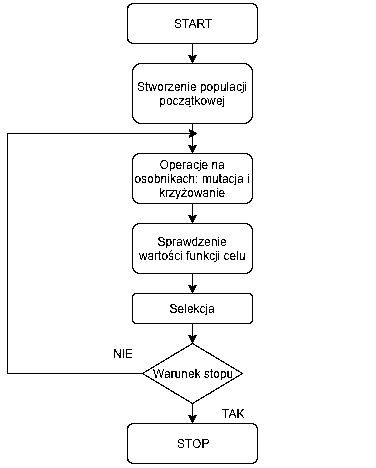
\includegraphics[scale=0.8]{ag}
		\centering
		\\
		{Rysunek1. Schemat algorytmu genetycznego} 
	\end{figure}	
	
	
	
	\begin{large}
		\begin{center}
			\textbf{Adaptacja algorytmu genetycznego}
		\end{center}
	\end{large}
	
	W pracy do problemu CVRP algorytm genetyczny został zaadaptowany w następujący sposób:
	
	\begin{center}
		\textbf{Reprezentacja rozwiązania}
	\end{center} 
	
	Każde rozwiązanie (osobnik) jest przedstawiony jako zbiór list punktów (miejsc) dla każdego pojazdu, ich współrzędne oraz ilość ładunku do wzięcia z danej lokalizacji, np. [[("BAZA", 10, 10), ("A", 15, 43, 5), ("B", 13, 54, 3), ("BAZA", 10, 10)] oznacza trasę biegnącą dla jednego pojazdu, która przedstawia się następująco następująo: START $\rightarrow$ A $\rightarrow$ B $\rightarrow$ KONIEC. Pierwsza dana w nawiasach oznacza nazwę lokalizacji, druga oznacza pierwszą współrzędną lokalizacji, następna liczba oznacza drugą współrzędną i na końcu ilość ładunku. Punkty "START" oraz "KONIEC" mają jednakowe współrzędne, gdyż flota pojazdów startuje w tego samego miejsca i do niego wraca. Punkty bazowe nie mają zdefiniowanych wartości ładunku do zabrania, gdyż baza jest jedynie miejscem startu i powrotu, a nie miejscem do odwiedzenia i zabrania ładunku (samochody startują z baz niezaładowane). Przykładowe rozwiązanie (jedynie z nazwami miejsc do odwiedzenia, w celu zwiększenia czytelności) przedstawiono na rys.1:
	
	\begin{figure}[h]
		\includegraphics[scale=0.8]{solution}
		\centering
		\\
		{Rysunek2. Ilustracja przykładowego rozwiązania}
	\end{figure}
	
	\newpage
	\begin{center}
		\textbf{Wygenerowanie populacji początkowej}
	\end{center}
	
	Na początku generowana jest losowo zadana liczba osobników, z których każdy spełnia wszystkie warunki do bycia rozwiązaniem w CVRP (tzn. każde miejsce jest odwiedzone tylko raz, początek i koniec trasy jest w tym samym punkcie, pojazdy muszą sumarycznie odwiedzić wszystkie lokalizacje, itd.). 
	
	\begin{center}
		\textbf{Selekcja}
	\end{center}

	Selekcja została przeprowadzona metodą rankingową, tzn. pozostaje odpowiednia liczba najlepszych osobników, pozostałę są odrzucane. W każdej iteracji programu wszystkie rozwiązania są sortowane na podstawie funkcji celu i z uporządkowanej listy odrzucane są najsłabsze osobniki, do dalszych operacji kwalifikują się te będące najwyżej w rankingu.
	
	\begin{center}
		\textbf{Krzyżowanie}
	\end{center}
	
	W krzyżowaniu przy powstawaniu nowego osobnika brane są pod uwagę dwie rzeczy: ilość punktów do odwiedzenia dla poszczególnych pojazdów oraz przebieg trasy dla każdego pojazdu. Najpierw dobierane są ilości miejsc do odwiedzenia na trasie dla poszczególnych pojazdów, a następnie dobierane są miejsca do odwiedzenia, zgodnie z ilością dla każdego pojazdu. Operacja krzyżowania została przeprowadzona w następujący sposób: \\
	1. Losowy wybór dwóch osobników, które będą rodzicami.\\
	2. Jeśli ilość pojazdów wynosi 1, wtedy ilość punktów do odwiedzenia dla dziecka jest taka sama jak dla rodziców (czyli wszystkie miejsca do odwiedzenia), w przeciwnym wypadku ilości miejsc do odwiedzenia dla kolejnych pojazdów wybierane są na przemian: raz z jednego rodzica, raz z drugiego (o ile wartości te spełniają warunki), na końcu (gdy już żadne wartości ilości punktów do odwiedzenia dla pojazdu nie spełniają warunków ) ustawiane są wartości losowe, dopełniające do ilości wszystkich miejsc do odwiedzenia, tak aby wszystkie miejsca zostały odwiedzone.\\
	3. Jeśli w punkcie poprzednim ilość pojazdów wynosiła 1, wtedy punkty do odwiedzenia są dobierane tak: od pierwszego rodzica jest brana pierwsza połowa trasy dla dziecka, od drugiego rodzica po kolei punkty do odwiedzenia w takiej kolejności w jakiej ma rodzic drugi, z uwzględnieniem faktu, że jedno miejsce można odwiedzić tylko jeden raz. Jeśli w punkcie poprzednim ilość pojazdów była większa niż 1, wtedy punkty dobierane są w taki sposób: dla pierwszego pojazdu brane są punkty do odwiedzenia (odpowiednia ilość kolejno od wszystkich pojazdów) od pierwszego rodzica, dla kolejnych od drugiego rodzica w analogiczny sposób. Całość jest sprawdzana pod kątem spełniania warunków- w przypadku, gdy warunki nie mogą zostać spełnione dane krzyżowanie jest pomijane i przechodzi się do następnego.\\
	
	\begin{center}
		\textbf{Mutacja}
	\end{center}

	Mutacja polega na losowej zamianie lokalizacji oraz ilości punktów do odwiedzenia dla poszczególnych pojazdów. W przypadku, gdy ilość pojazdów wynosi 1, oczywiście ilość punktów do odwiedzenia dla tego pojazdu jest równa ilości wszystkich punktów do odwiedzenia. Wtedy losowo zmieniana jest tylko kolejność punktów do odwiedzenia poprzez znalezienie innej permutacji tych punktów. W przypadku, gdy ilość pojazdów jest większa niż 1, wtedy ilości punktów dla poszczególnych pojazdów w rozwiązaniu są wybierane w sposób losowy przy uwzględnieniu ograniczeń, tzn. ilość pojazdów się nie zmienia oraz wszystkie punkty muszą zostać odwiedzone dokładnie jeden raz. Następnie kolejność punktów do odwiedzenia jest losowo zamieniane poprzez znalezienie innej permutacji oraz punkty kolejno są przydzielane do pojazdów przy uwzględnieniu ograniczeń wynikających z ładowności pojazdu. Jeśli warunki nie mogą zostać spełnione dana mutacja jest pomijana.
	
	\begin{center}
		\textbf{Warunek stopu}
	\end{center}

	Warunkiem stopu jest wykonanie odpowiedniej ilości iteracji algorytmu. Przykładowo dla wartości 100, program wykona w pętli 100 razy procesy krzyżowania, mutacji i selekcji, a następnie przejdzie do wyboru najlepszego osobnika.\\
	
	\newpage
	\begin{flushleft}
		\begin{LARGE}
			\textbf{4. Opis projektu}
		\end{LARGE}
	\end{flushleft}
	
	\vspace{5mm} %5mm vertical space
	
	\begin{flushleft}
		\begin{large}
			\textbf{4.1. Użyte technologie}
		\end{large}
	\end{flushleft}
	\vspace{10mm} %5mm vertical space
	
	 Aplikacja została utworzona w języku programowania python (z użyciem dostępnych bibliotek) oraz przy użyciu ogólnie dostępnych map OSM (OpenStreetMap).\\
	 Na podstawie \hyperlink{python}{[4]}:\\
	 \textbf{Python}- jest językiem programowania ogólnego przeznaczenia. Jest to język wysokiego poziomu. Może być skutecznie wykorzystywany przy budowie w zasadzie każdego programu. Nie potrzebuje bezpośredniego dostępu do sprzętu komputerowego. Python nie jest optymalny dla programów, które mają duże ograniczenia niezawodności lub są zbudowane i utrzymywane przez wiele osób lub przez długi czas. Ma on jednak kilka zalet w porównaniu z innymi językami programowania, m.in.:\\
	 - jest łatwy w nauce\\ 
	 - posiada bardzo dużą liczbę darmowych i powszechnie dostępnych bibliotek, zapewniających rozszerzoną funkcjonalność\\ 
	 
	 Na podstawie \hyperlink{osm}{[5]}:\\
	 \textbf{OSM (OpenStreetMap)}- jest to darmowa, edytowalna mapa całego świata, tworzona przez wolontariuszy, wydawana na licencji open-content. Licencja OpenStreetMap pozwala na bezpłatny dostęp do obrazów i podstawowych danych map. Projekt ma na celu promowanie nowych zastosowań tych danych. W pracy OSM zostało wykorzystane do zwizualizowania przebiegów tras i pokazania ich na rzeczywistej mapie. Przykład obrazu uzyskanego dzięki OSM \hyperlink{osm_photo}{[6]}: \\
	 
 	\begin{figure}[h]
 	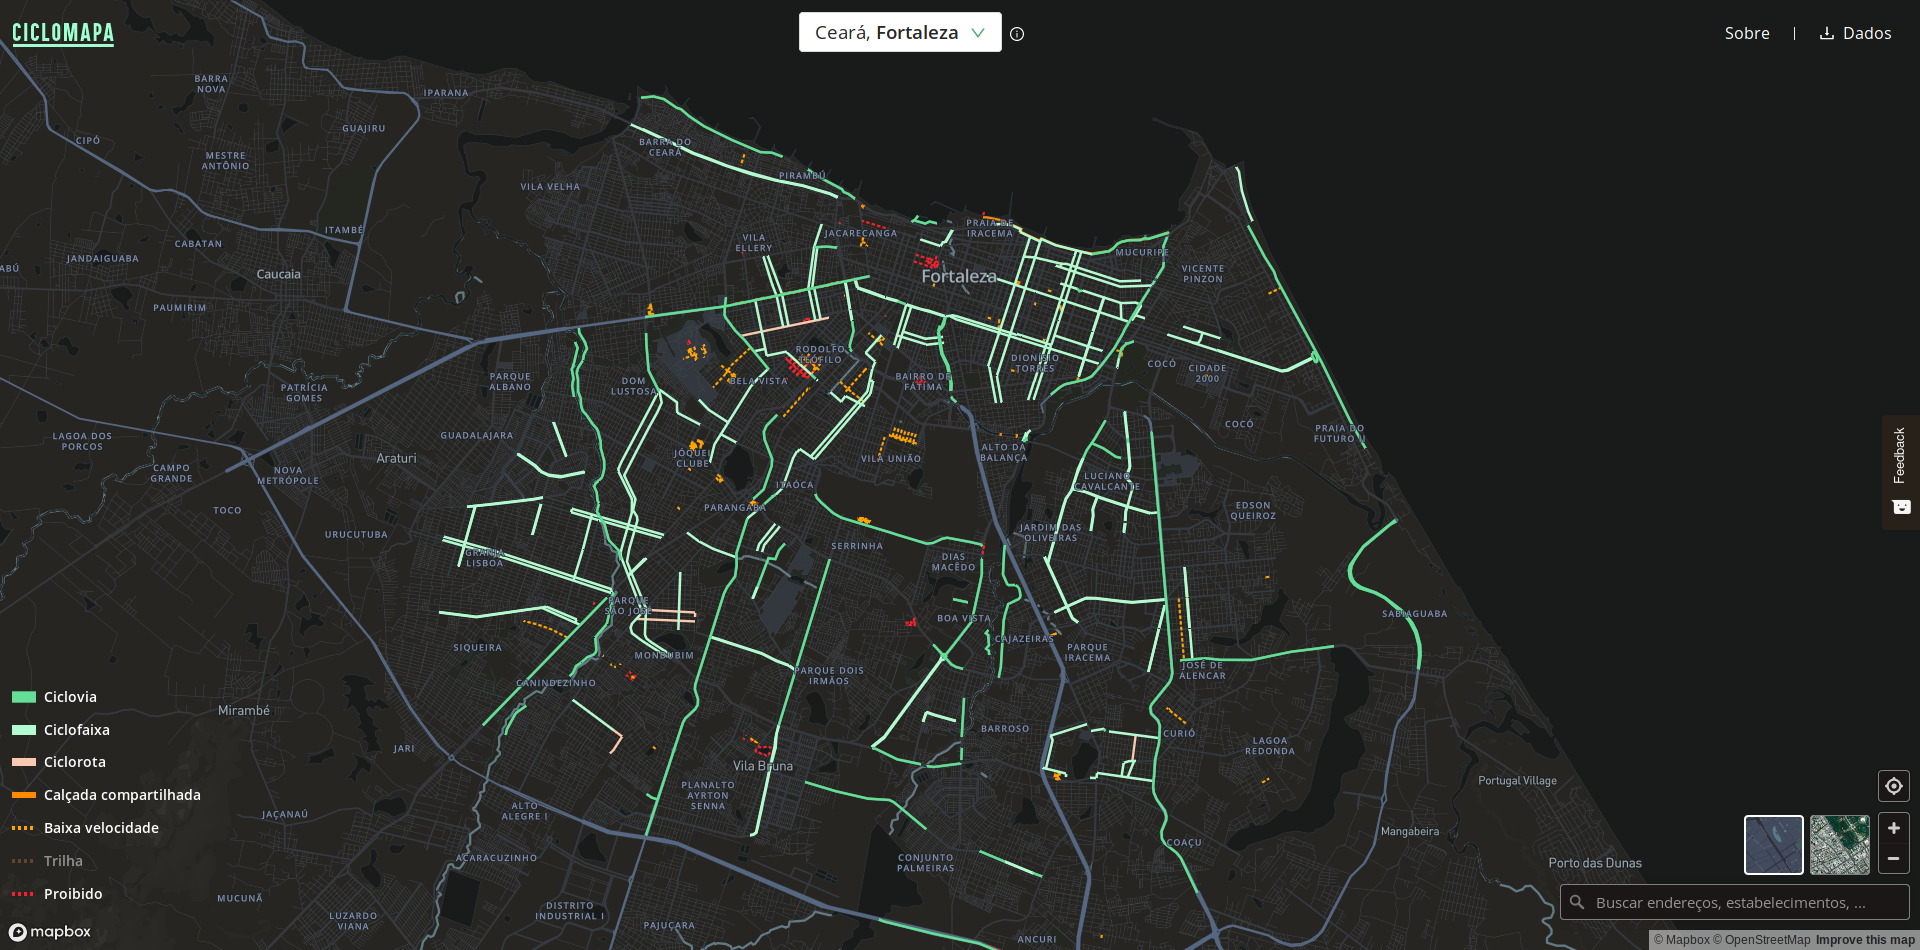
\includegraphics[scale=0.23]{osm_example}
 	\centering
 	\\
 	{Rysunek2. Przykładowy screen z osm}
	\end{figure}
	 
	 Poniżej przedstawiono krótki opis najważniejszych bibliotek użytych do stworzenia programu w języku python: \\
	 
	 
	 Na podstawie \hyperlink{pyqt}{[5]}:\\
	 PyQt- jest to zbiór bibliotek pythona stworzonych przez Riverbank Computing. Służą do tworzenia interfejsów graficznych aplikacji w ramach międzyplatformowego frameworka Qt, który jest open-sourcowy. Możliwa w użyciu na wielu systemach opercyjnych i platformach. W programie została użyta w celu zrobienia GUI oraz wyświetlania w nim mapy.\\
	 
	 
	 Na podstawie \hyperlink{folium}{[5]}:\\
	 Folium- w znacznym stopniu opiera się na bibliotece leaflet.js służącej do mapowania, tworzenia interaktywnych map w javascript. Folium pozwala na przetwarzanie danych geograficznych oraz ich wizualizację w pythonie. W aplikacji za pomocą tej biblioteki tworzone są mapy w formacie html, które następnie są wyświetlane w gui stworzonym przy pomocy PyQt.\\
	 
	 \begin{figure}[h]
	 	\includegraphics[scale=0.8]{folium}
	 	\centering
	 	\\
	 	{Rysunek3. Przykładowa mapa interaktywna stworzona przy użyciu folium\hyperlink{folium}{[5]}}
	 \end{figure}
	 
	 Na podstawie \hyperlink{geopy}{[5]}:\\
	 Geopy- biblioteka pozwalająca na łatwą lokalizację współrzędnych geograficznych na podstawie adresów oraz obliczania odległości na globie między dwoma zbiorami współrzednych (długość i szerokość geograficzna). W pracy użyta w celu obliczenia odległości na globie dla zestawu danych.\\
	 
	 
	 Na podstawie \hyperlink{json}{[5]}:\\
	 Json- biblioteka służąca do kodowania i dekodowania danych w formacie json. JSON (JavaScript Object Notation) to format wymiany danych. Jest to format niezależny od języka programowania. Opiera się na dwóch danych: nazwa i wartość. W pracy biblioteka json została wykorzystana do dekodowania danych wejściowych zapisanych w formacie json i zapisywania ich w pythonowej strukturze danych OrderedDict().\\
	 
	
	
	\newpage
	
	
	\begin{flushleft}
		\begin{large}
			\textbf{4.2. Opis aplikacji}
		\end{large}
	\end{flushleft}
	\vspace{10mm} %5mm vertical space
	
	Główna (z perspektywy użytkownika) część aplikacji czyli GUI (Graphical User Interface) została wykonana, jak wspomniano w poprzednim rozdziale z użyciem biblioteki PyQt. Najważniejszym celem aplikacji jest stworzenie prostego w użyciu środowiska do obliczania optymalnej trasy dla problemu CVRP. Program jest łatwy i intuicyjny w użyciu dzięki stworzonemu panelowi graficznemu, który pozwala na dobór odpowiednich opcji. Pod warstwą graficzną kryje się oczywiście kod programu odpowiadający za implementację algorytmu genetycznego i znalezienie trasy optymalnej przy odpowiednich ograniczeniach. Wynik zostaje przedstawiony w formie graficznej na mapie interaktywnej.

	\begin{large}
		\begin{center}
			\textbf{Okno główne}
		\end{center}
	\end{large}

	\begin{figure}[h]
		\includegraphics[scale=0.9]{gui}
		\centering
		\\
		{Rysunek4. Okno programu}
	\end{figure}
	
	Z perspektywy użytkownika GUI (Graphical User Interface) to najważniejszy element, który pozwala na sprawne korzystanie z aplikacji. Okno programu umożliwia podanie parametrów istotnych z punktu widzenia problemu CVRP oraz algorytmu genetycznego, takich jak: \\
	- ilość pojazdów (number of vehicles)\\
	- pojemność pojazdów (vehicles capacity)\\
	- nazwa punktu bazowego\\
	- współrzędne bazy (rozdzielone przecinkiem)\\
	- prawdopodobieństwo krzyżowania (crossing probability)\\
	- prawdopodobieństwo mutacji (mutation probability)\\
	- ilość osobników w pokoleniu początkowym (number of individuals in first generation)\\
	- ilość najlepszych osobników wyłanianych w rankingu (number of individuals to stay)\\
	- ilość iteracji AG (number of iterations)\\
	
	Opis okna:
	
	\begin{itemize}
		\item Domyślnymi wartościami powyżej przedstawionych parametrów są te przedstawione na rys.4.
		\item Po lewej stronie GUI znajduje się lista punktów do odwiedzenia (wczytywana z pliku o rozszerzeniu .json), które można zaznaczać i odznaczać, tzw. checkboxes. Punkty zaznaczone to te, które będą uwzględniane w programie przy wyborze tras.
		\item W dolnej części GUI znajduje się przycisk "Calculate track", który po wciśnięciu uruchamia proces obliczeniowy, wybierający optymalną trasę. Następnie najlepsze rozwiązanie jest przedstawione na interaktywnej mapie.
		\item Po prawej stronie przycisku znajduje się pole wynikowe "Result". Wyświetla ono najlepszą znalezioną wartość funkcji celu, tzn. wartość funkcji celu dla najlepszego osobnika.
	\end{itemize}

	\begin{large}
		\begin{center}
			\textbf{Mapa}
		\end{center}
	\end{large}
	
	Punkty na mapie są oznaczone specjalnymi znacznikami. Kolorem czerwonym została oznaczona baza, czyli punkt początkowy i końcowy dla każdej trasy, a kolorem zielonym pozostałe punkty. Każda trasa jest oznaczona innym, losowym kolorem. Punkty na trasie są połączone linią prostą ilustrującą kolejność punktów na trasie. Linia ta pokazuje połączenie między dwoma kolejnymi punktami. Ze względu na fakt, że odległości są obliczane przy pomocy funkcji geodesic() z biblioteki geopy, która liczy najkrótszą odległość między punktami na kuli ziemskiej, można przyjąć, że otrzymana trasa jest dobrym przybliżeniem najkrótszej trasy przy poruszaniu się środkiem lokomocji takim jak samolot lub helikopter.
	Poniżej przedstawiono przykładową mapę ilustrującą połączenia między punktami, dla zadanych miejsc:
	
	\newpage
	\begin{figure}[h]
		\includegraphics[scale=0.8]{map}
		\centering
		\\
		{Rysunek5. Wyświetlana mapa}
	\end{figure}
	
	Po kliknięciu na ikonę miejsca wyświetlana jest jego nazwa:
	
	\newpage
	
	\begin{figure}[h]
		\includegraphics[scale=0.8]{miejsce}
		\centering
		\\
		{Rysunek6. Wyświetlana nazwa miejsca}
	\end{figure}
	
	
	\newpage
	\begin{flushleft}
		\begin{LARGE}
			\textbf{5. Testy}
		\end{LARGE}
	\end{flushleft}

	Testy dla CVRP przy użyciu algorytmu genetycznego zostały przeprowadzone dla danych uzyskanych z \hyperlink{tests}{[5]}. Ze względu na stukturę plików testowych poniższe testy są przeprowadzone dla punktów na płaszczyźnie XY. Odległość między punktami jest liczona jako pierwiastek z sumy kwadratów różnic między współrzędnymi x oraz y, tzn. odległość = $\sqrt{(x_1-x_2)^2 + (y_1-y_2)^2}$.
	
	\begin{flushleft}
		\begin{large}
			\textbf{5.1. Instancja testowa 1}
		\end{large}
	\end{flushleft}
	\vspace{10mm} %5mm vertical space
	
	Pierwszy instancję testową stanowi pierwszy plik z Set A, tzn. A-n32-k5 (patrz \hyperlink{tests}{[5]}).
	Jest to zbiór 32 punktów (włącznie z bazą), dla którego najlepszym znalezionym rozwiązaniem jest wartość 784. 
	
	
	
	\newpage
	
	\renewcommand\refname{Źródła}
	\begin{thebibliography}{}

		\bibitem{komiwojazer} 
		{\hypertarget{komiwojazer}{\textcolor{blue}{
		Sysło M.M., Deo N., Kowalik J.S., Algorytmy optymalizacji dyskretnej, wyd. drugie, Warszawa: Wydawnictwo Naukowe PWN, 1995, ISBN 83-01-11818-0}}}
	
		\bibitem{tsp_math_model}
		{\hypertarget{tsp_math_model}{Materiały dostępne na stronie: \textcolor{blue}{
		http://examples.gurobi.com/traveling-salesman-problem/}, dostęp we wrześniu 2019r.}}
	
	 
	 	\bibitem{vrp_all}
	 	{\hypertarget{vrp_all}{\textcolor{blue}{
		https://www.researchgate.net/publication/313005083\_Vehicle\_routing\_problem\_Models\_and\\\_solutions}}}
		
		\bibitem{cvrp-irnich} 
		{\hypertarget{cvrp-irnich}{\textcolor{blue}{https://www.researchgate.net/publication/284529903\_Chapter\_1\_The\_Family\_of\_Vehicle\_\\Routing\_Problems}}}
		
		\bibitem{vrp_variants} 
		{\hypertarget{vrp_variants}{\textcolor{blue}{http://www.vrp-rep.org/variants.html}}}
		
		\bibitem{vrp_solving} 
		{\hypertarget{vrp_solving}{\textcolor{blue}{https://en.wikipedia.org/wiki/Vehicle\_routing\_problem}}}
		
		\bibitem{metaheurystyka} 
		{\hypertarget{metaheurystyka}{\textcolor{blue}{Bianchi, Leonora; Marco Dorigo; Luca Maria Gambardella; Walter J. Gutjahr (2009). "A survey on metaheuristics for stochastic combinatorial optimization"}}}
		
		\bibitem{algorithm} 
		{\hypertarget{algorithm}{\textcolor{blue}{
		Thomas H. Cormen; Charles E. Leiserson; Ronald L. Rivest; Clifford Stein (2009). Introduction To Algorithms (3rd ed.). MIT Press. ISBN 978-0-262-03384-8.}}}
		
		
		\bibitem{ant} 
		{\hypertarget{ant}{\textcolor{blue}{
		https://www.sciencedirect.com/topics/engineering/ant-colony-optimization}}}
	
		\bibitem{bees} 
		{\hypertarget{bees}{\textcolor{blue}{
		http://www.cleveralgorithms.com/nature-inspired/swarm/bees\_algorithm.html}}}
	
		\bibitem{bees_code} 
		{\hypertarget{bees_code}{\textcolor{blue}{
		https://www.ncbi.nlm.nih.gov/pmc/articles/PMC4553508/}}}

		
		\bibitem{ag} 
		{\hypertarget{ag}{\textcolor{blue}{
		D. E. Goldberg: Algorytmy genetyczne i ich zastosowania. Warszawa: WNT, 1998. (pol.)}}}
	
		\bibitem{ag_operators} 
		{\hypertarget{ag_operators}{\textcolor{blue}{
		https://www.tutorialspoint.com/genetic\_algorithms/index.htm}}}
	
		\bibitem{cross} 
		{\hypertarget{cross}{\textcolor{blue}{
		https://www.tutorialspoint.com/genetic\_algorithms/genetic\_algorithms\_crossover.htm}}}
	
		\bibitem{mutation} 
		{\hypertarget{mutation}{\textcolor{blue}{
		https://towardsdatascience.com/introduction-to-genetic-algorithms-including-example-code-e396e98d8bf3}}}
	
		\bibitem{selection} 
		{\hypertarget{selection}{\textcolor{blue}{
		https://www.tutorialspoint.com/genetic\_algorithms/genetic\_algorithms\_parent\_selection.htm}}}
	
		\bibitem{python} 
		{\hypertarget{python}{\textcolor{blue}{
		 Guttag, John V. (12.08.2016). Introduction to Computation and Programming Using Python: With Application to Understanding Data. MIT Press. ISBN 978-0-262-52962-4.}}}
	 
	 	\bibitem{osm} 
	 	{\hypertarget{osm}{\textcolor{blue}{
		https://wiki.openstreetmap.org/wiki/About\_OpenStreetMap}}}
		
		
		\bibitem{osm_photo} 
		{\hypertarget{osm_photo}{\textcolor{blue}{
		https://wiki.openstreetmap.org/wiki/File:Screenshot\_2019-10-23\_CicloMapa.png
		}}}
	
		\bibitem{pyqt} 
		{\hypertarget{pyqt}{\textcolor{blue}{
		https://python101.readthedocs.io/pl/latest/pyqt/
		}}}
	
	
		\bibitem{folium} 
		{\hypertarget{folium}{\textcolor{blue}{
		https://python-visualization.github.io/folium/
		}}}
	
		\bibitem{geopy} 
		{\hypertarget{geopy}{\textcolor{blue}{
		https://geopy.readthedocs.io/en/stable/
		}}}
	
		\bibitem{json} 
		{\hypertarget{json}{\textcolor{blue}{
		https://www.json.org/json-pl.html
		}}}
	
		\bibitem{tests} 
		{\hypertarget{tests}{\textcolor{blue}{
		http://neo.lcc.uma.es/vrp/vrp-instances/capacitated-vrp-instances/http://neo.lcc.uma.es/vrp/vrp-instances/capacitated-vrp-instances/
		}}}
	
		

	\end{thebibliography}
	
	
	%\end{flushleft}
	
\end{document}